\documentclass[runningheads]{llncs}
\usepackage{graphicx}
\usepackage{epsfig}
\usepackage{xspace}
\usepackage{amssymb}
\usepackage{listings}

\newcommand{\sgr}[1]{\textbf{sgr: {#1}}}
\newcommand{\wsml}[1]{\begin{scriptsize}{\sf {\bf #1}}\end{scriptsize}}

% WSML language keywords; and general syntax (for inline usage)
\newcommand{\synkw}[1]{\textsf{\small \textbf{#1}}}
\newcommand{\syn}[1]{\textsf{\small #1}}


\begin{document}

%%%%%%%%%%%%%%%%%%%%%%%%%%%%%%%%%%%%%%%%%%%%%%
%wsmo listings
\lstdefinelanguage{MOF}{
  alsodigit=-,%
  morekeywords={Class,type,multiplicity,single-valued,sub-Class},
  sensitive=true
}

\lstdefinestyle{mof}{
 language=MOF,
 basicstyle=\scriptsize\sffamily,
 keywordstyle=\bfseries,
 showstringspaces=false,
 flexiblecolumns=true,
 frame=tb,
 xleftmargin=15pt,
 xrightmargin=15pt,
}

%wsml listing
\lstdefinelanguage{WSML}{
  morekeywords={wsmlVariant,namespace,nonFunctionalProperties,endNonFunctionalProperties,importsOntology,
    usesMediator,ontology,goal,ooMediator,ggMediator,wgMediator,wwMediator,webService,concept,
    subConceptOf,ofType,impliesType,transitive,symmetric,inverseOf,reflexive,relation,subRelationOf,
    function,instance,relationInstance,memberOf,hasValue,axiom,definedBy,source,target,useService,
    capability,precondition,postcondition,assumption,effect,interface,choreography,orchestration,
    exists, forAll, implies, impliedBy, equivalent},
  sensitive=true,
  morestring=[b]",morestring=[d]�,
  morecomment=[s]{/*}{*/},
}

\lstdefinestyle{wsml}{
 language=WSML,
 basicstyle=\scriptsize\sffamily,
 keywordstyle=\bfseries,
 showstringspaces=false,
 mathescape=true,
 flexiblecolumns=true,
 frame=tb,
 xleftmargin=15pt,
 xrightmargin=15pt,
}


\lstdefinestyle{xml}{
 language=XML,
 basicstyle=\scriptsize\sffamily,
 keywordstyle=\bfseries,
 showstringspaces=false,
 mathescape=true,
 frame=tb,
 flexiblecolumns=true,
 xleftmargin=15pt,
 xrightmargin=15pt,
}

\lstdefinestyle{wsml-table}{
 language=WSML,
 basicstyle=\scriptsize\sf,
 keywordstyle=\bfseries,
 showstringspaces=false,
 mathescape=true,
 flexiblecolumns=true,
 %frame=tb,
 breaklines=true,
 captionpos=b,
 xrightmargin=5pt,
 xleftmargin=5pt,
}


\title{A Reasoning Framework for Rule-Based WSML}

\author{Stephan Grimm\inst{1} \and Uwe Keller\inst{2} \and Holger Lausen\inst{2} \and G\'abor Nagyp\'al\inst{1}\newline\textbf{order of authors is currently alphabetic}}
\institute{
    FZI Research Center for Information Technologies at the University of Karlsruhe\\
    Karlsruhe, Germany\\
    \email{$\{$grimm,nagypal$\}$@fzi.de}\\
\and
    Digital Enterprise Research Institute\\
    Innsbruck, Austria\\
    \email{$\{$keller,lausen$\}$@deri.org}\\
}

\maketitle

\begin{abstract}
%The use of ontology languages for semantically annotating Web
%Services demands for reasoning support in order to facilitate
%tasks like automated discovery or composition of services based on
%semantic descriptions of their functionality.
WSML is an ontology language specifically tailored to annotate Web
Services, and part of its semantics adheres to the rule-based
knowledge representation paradigm of logic programming. We present a
framework to support reasoning with rule-based WSML language
variants based on existing Datalog inference engines. Therein, the
WSML reasoning tasks of knowledge base satisfiability and instance
retrieval are implemented through a language mapping to Datalog
rules and Datalog querying. Part of the WSML semantics is realized
by a fixed set of rules that form meta-level axioms. Furthermore,
the framework exhibits some debugging functionality that allows for
identifying violated constraints and for pointing out involved
instances and problem types. Its highly modular architecture
facilitates easy extensibility towards other language variants and
additional features. The available implementation of the framework
provides the first reasoners for the WSML language.

\end{abstract}

\section{Motivation\label{sec:motivation}}
-- motivate the provision of reasoning support for (rule-based) WSML based on existing inference engines \\
-- stress that this is the first specific WSML Reasoner implementation available \\

\section{Reasoning in the WSML Language\label{sec:wsml}}
-- give an overview of the WSML language; focus on semantics of rule-based variants (also show how syntax looks like, e.g. by an example) \\
-- focus on the ontology language part of WSML (only briefly mention WS-specific parts) and sketch its features, such as constraints, datatypes, conceptual modelling + axiomatic formulations, ... \\
-- describe the reasoning tasks in WSML, i.e. KB satisfiability and entailment \\
-- relate language features and reasoning, e.g. constraints and satisfiability, to emphasise the close connection of these features to reasoning \\

\newcommand{\smtxtit}[1]{\begin{scriptsize}\ensuremath{\textit{#1}}\end{scriptsize}}
\newcommand{\trans}[1]{\ensuremath{\tau_{#1}}\xspace}
\newcommand{\transtxt}[1]{\trans{\smtxtit{#1}}}
%\newcommand{\transmap}[3]{\ensuremath{\tau_{#1}^{{#2},{#3}}}\xspace}
%\newcommand{\transtxtmap}[3]{\transmap{\smtxtit{#1}}{#2}{#3}}
\def\LE{\ensuremath{\mathcal{L\!E}}\xspace}
\def\O{\ensuremath{\mathcal{O}}\xspace}
\def\P{\ensuremath{\mathcal{P}}\xspace}
\newcommand{\powset}[1]{\ensuremath{2^{#1}}\xspace}

% -- meta-level predicates
\newcommand{\predicate}[1]{\ensuremath{p_{#1}}\xspace}
\newcommand{\predsubtxt}[1]{\mathrm{\tt #1}}
\def\psco{\predicate{\predsubtxt{sco}}}
\def\pmo{\predicate{\predsubtxt{mo}}}
\def\phval{\predicate{\predsubtxt{hval}}}
\def\pitype{\predicate{\predsubtxt{itype}}}
\def\potype{\predicate{\predsubtxt{otype}}}

\section{Realistion of WSML Reasoning through a Mapping to Datalog\label{sec:mapping}}
-- briefly sketch the idea of reasoning via rule based inferencing \\

The semantics of rule-based WSML is defined via a mapping to
datalog with (in)equality and integrity constraints. \sgr{probably
use a special denotation like $\textit{datalog}^{!=,IC}$, which
then has to be introduced in Section 2} Thus, the reasoning
framework performs various transformations to convert an original
ontology in WSML syntax into datalog rules. To maintain the
semantics of more complex WSML language constructs that cannot
directly be expressed in datalog, a fixed set of rules form the
meta-level axioms that realise part of the WSML semantics during
reasoning. Finally, the WSML reasoning tasks of knowledge base
satisfiability and instance retrieval are realised by datalog
querying via calls to an underlying datalog inference engine that
is fed with the rules produced during transformation together with
the meta-level axioms.

\subsection{Transformation of WSML into Datalog}
-- describe different transformation steps \\

The transformation of a WSML ontology to datalog rules forms a
pipeline of single transformation steps which are subsequently
applied, starting from the original ontology.

\paragraph{Axiomatization} -- In a first step, the transformation
\transtxt{axiom} is applied as a mapping $\O \mapsto \powset{\LE}$
from the set of all valid ontologies formulated in rule-based WSML
to the powerset of all logical expressions that conform to
rule-based WSML. \transtxt{axiom} converts all conceptual syntax
elements, such as concept and attribute definitions or cardinality
and type constraints, into appropriate logical expressions
according to \cite{wsml-spec}(Table 8.1). \sgr{give the complete
conversion table ??}

To give an example, the WSML fragment
\begin{lstlisting}[style=wsml]
concept C subConceptOf D
    r ofType (0 2) T
instance a memberOf C
    r hasValue b,c
\end{lstlisting}
is translated by \transtxt{axiom} to the following logical
expressions.
\begin{lstlisting}[style=wsml]
C subConceptOf D. C[r ofType T].
!- ?x memberOf C and ?x[r hasValue?y1, r hasValue ?y2] and ?y1 != ?y2.
a memberOf C.  a hasValue b,c.
\end{lstlisting}

\paragraph{Normalization} -- The transformation \transtxt{norm} is
applied to normalize WSML logical expressions as a mapping
$\powset{\LE} \mapsto \powset{\LE}$. This normalization step
reduces the complexity of WSML logical expressions according to
\cite{wsml-spec}(Section 8.2) to make them better fit the simple
syntactic form of literals in datalog rules. This reduction
includes conversion to negation and disjunctive normal forms as
well as decomposition of complex WSML molecules (see
\cite{wsml-spec}).

\paragraph{Lloyd-Topor Transformation} -- The transformation
\transtxt{Lloyd-Topor} is applied as a mapping $\powset{\LE}
\mapsto \powset{\LE}$ to flatten the complex WSML logical
expressions, producing simple rules according to the Lloyd-Topor
transformations \cite{lloyd-topor} as follows.

\begin{center}
\begin{tabular}{|c|c|}
  \hline
  % after \\: \hline or \cline{col1-col2} \cline{col3-col4} ...
  \emph{original expression} & \emph{simplified rule(s)} \\
  \hline
  $H_1 \wedge \dots \wedge H_n \leftarrow B$ & $H_1 \leftarrow B , \dots , H_n \leftarrow B$ \\
  $H_1 \leftarrow H_2 \leftarrow B$ & $H_1 \leftarrow H_2 \wedge B$ \\
  $H \leftarrow B_1 \vee \dots \vee B_n$ & $H \leftarrow B_1 , \dots , H \leftarrow B_n$ \\
  \hline
\end{tabular}
\end{center}

After this step, the resulting WSML expressions have the form of
proper datalog rules with a single head and conjunctive (possibly
negated) body literals.

\paragraph{Datalog Rule Generation} -- In a final step, the
transformation \transtxt{datalog} is applied as a mapping
$\powset{\LE} \mapsto \P$ from all valid logical expressions in
rule-based WSML to the set of all datalog programs, yielding
generic datalog rules that represent the content of the original
WSML ontology. In this generic datalog program, all remaining
WSML-specific language constructs, such as \wsml{subConceptOf} or
\wsml{ofType}, are replaced by special meta-level predicates for
which the semantics of the respective language construct is
encoded in meta-level axioms as described in a further subsection.
\begin{table}[b]\label{tab:LE2datalog}\centering
\begin{tabular}{|l|c|}
  \hline
  bla & bla \\
  \hline
\end{tabular}
\caption{Transformation from logical expressions in rule-based
WSML to datalog including meta-level predicates.}
\end{table}
Table \ref{tab:LE2datalog} shows the mapping from WSML logical
expressions to generic datalog including such meta-level
predicates.

Notice that the \wsml{memberOf} construct for instantiation is
also mapped to an appropriate meta-level predicate instead of
direct instantiation of the form $C(i)$, which is available in
datalog. This decision was taken in order to facilitate the
metamodelling capabilities of rule-based WSML, which allows an
entity to be both an instance and class at the same time.
\sgr{genauer darstellen f�r was welche metal-level Predikate
erzeugt werden!}

\bigskip

Ultimately, the basic transformation pipeline for converting a
rule-based WSML ontology into a datalog program is the following,
constituted by the single transformation steps introduced before.
\begin{displaymath}
    \tau = \transtxt{datalog} \circ \transtxt{Lloyd-Topor} \circ \transtxt{norm} \circ \transtxt{axiom}
\end{displaymath}
As a mapping $\O \mapsto \P$, this chaining of the single steps is
applied to a WSML ontology $O \in \O$ to yield a semantically
equivalent datalog program $\tau (O) = P \in \P$ when interpreted
with respect to the meta-level axioms discussed next.

\subsection{Realising WSML Semantics through Meta Axioms}
-- describe how a fixed set of rules implements (part of) the WSML semantics during reasoning \\

The mapping from WSML to datalog in the reasoning framework works
such that each WSML-identifiable entity, i.e. concepts, instances,
attributes etc., is mapped to an instance (or logical constant) in
datalog, as depictef in Figure \ref{fig:meta}. There, the concepts
$C_1, C_2$ as well as the instances $I_1, I_2$ and the attribute
$a$ are mapped to constants such as $I_{C_1}$, $I_{I_1}$ or $I_a$
in datalog, representing the original WSML entities on the
instance level.

Accordingly, the various special-purpose relations that hold
between WSML entities, such as \wsml{subConceptOf},
\wsml{memberOf} or \wsml{hasValue}, are mapped to datalog
predicates that form a meta-level vocabulary that reflects the
WSML language constructs. They are applied to the datalog
instances that represent the WSML concepts instances and
attributes. Table \ref{tab:meta-level} shows all the meta-level
predicates together with the WSML language construct they stand
for. The facts listed in Figure \ref{fig:meta} illustrate the use
of the meta-level predicates. For example, the predicate \psco
takes two datalog constants as arguments that represent WSML
concepts to state that the concept represented by the first
argument is a subconcept of the one represented by the second
argument; on the other hand, the predicate \pmo takes a datalog
constant that represents a WSML instance and one that represents a
WSML concept to state that the instance is in the extension of
this concept.

In contrast to a direct mapping from WSML to datalog with
concepts, attributes and instances mapping to unary predicates,
binary predicates and constants, respectively, this indirect
mapping allows for the WSML metamodelling facilities.
Metamodelling allows an entity to be a concept and an instance at
the same time. By representing a WSML entity as a datalog
constant, it could, for example, fill both the first as well as
the second argument of e.g.\ the predicate \pmo, in which case it
is interpreted as both an instance and a concept.

\begin{figure}[tb]
        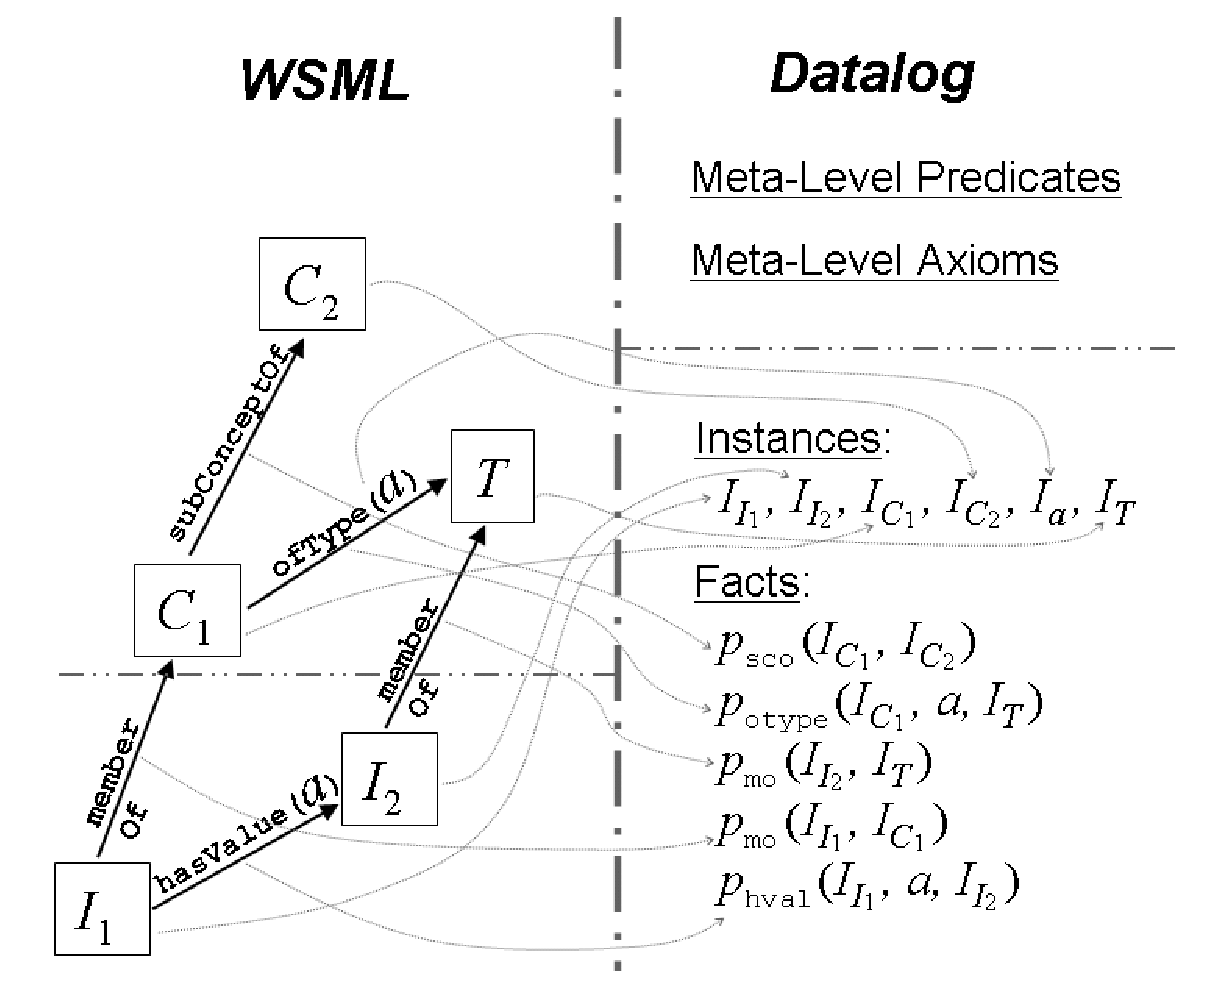
\includegraphics[width=8cm]{figures/meta}
        \centering
    \caption{Meta-level predicates and axioms for realising the WSML semantics. \label{fig:meta}}
\end{figure}


\def\filler{\phantom{l}}
\begin{table}[tb]\label{tab:meta-level}\centering
\begin{tabular}{|l|l|}
  \hline
  \multicolumn{2}{|l|}{\emph{Meta-Level Predicates}} \\
  \filler \begin{small}Predicate\end{small} & \begin{small}WSML construct\end{small} \\
  \hline
  \filler $\psco(C_{sub},C_{sup})$ \qquad\qquad & $C_{sub}$ \wsml{subConceptOf} $C_{sup}$ \\
  \filler $\pmo(I,C)$ & $I$ \wsml{memberOf} $C$ \\
  \filler $\phval(I,a,V)$ & $I[a$ \wsml{hasValue} $V]$ \\
  \filler $\pitype(C,a,T)$ & $C[a$ \wsml{impliesType} $T]$ \\
  \filler $\potype(C,a,T)$ & $C[a$ \wsml{ofType} $T]$ \\
  \hline\hline
  \multicolumn{2}{|l|}{\emph{Meta-Level Axioms}} \\
  \hline
  \multicolumn{2}{|l|}{\filler $\psco(C_1,C_3) \leftarrow \psco(C_1,C_2) \wedge \psco(C_2,C_3)$} \\
  \multicolumn{2}{|l|}{\filler $\pmo(I,C_2) \leftarrow \pmo(I,C_1) \wedge \psco(C_1,C_2)$} \\
%  \multicolumn{2}{|l|}{\filler $\pmo(V,C_2) \leftarrow \pitype(C_1,a,C_2) \wedge \pmo(I,C_1) \wedge \phval(I,a,V)$} \\
  \multicolumn{2}{|l|}{\filler $\pmo(V,C_2) \leftarrow \pitype(C_1,a,C_2) \wedge \pmo(I,C_1)$} \\
  \multicolumn{2}{|l|}{\filler \phantom{$\pmo(V,C_2) \leftarrow$} \qquad $\wedge \phval(I,a,V)$} \\
%  \multicolumn{2}{|l|}{\filler $ \leftarrow \potype(C_1,a,C_2) \wedge \pmo(I,C_1) \wedge \phval(I,a,V) \wedge \neg \pmo(V,C_2)$} \\
  \multicolumn{2}{|l|}{\filler $ \leftarrow \potype(C_1,a,C_2) \wedge \pmo(I,C_1)$} \\
  \multicolumn{2}{|l|}{\filler $ \phantom{\leftarrow} \qquad \wedge \phval(I,a,V) \wedge \neg \pmo(V,C_2)$} \\
 \hline
\end{tabular}
\caption{Meta-level axioms and predicates for WSMl semantics in
datalog.}
\end{table}


\subsection{Mapping WSML Reasoning Tasks to Datalog Querying}
-- describe how to realise WSML satisfiability and entailment to datalog querying \\

\subsection{Realising Datatype Reasoning}
-- describe how reasoning with datatypes is realised

\section{Debugging Support\label{sec:debugging}}
-- briefly motivate debugging features for the ontology engineering process \\

\subsection{Debugging Features to Support Ontology Development}
-- describe the kind of debugging features the framework supports and what they allow for \\

\subsection{Realisation of Debugging Features through Meta Axioms}
-- describe how these debugging features are realised via an additional fixed set of rules \\

\section{Reasoning Framework Overview\label{sec:framework}}

The design goals of our framework are modularity for the
transformation steps and flexibility with respect to the
underlying inference engine. The modularity allows to reuse
transformation functionality across different WSML variants and
reduces the effort for accomplishing other reasoning tasks. By
reducing WSML to simple Datalog constructs and providing a
respective object model we have reduced the effort of integrating
new reasoners to a minimum\footnote{In fact, the adaptation of the
framework to the MINS rule engine took less then a day.}.

\subsection{Architecture and Internal Layering}
Figure~\ref{fig:layering} shows the basic components of the system
\sgr{it is not clear what "the system" is here.} as well as the
data flow during a prototypical usage scenario. The inner box
shows the currently implemented transformations that are bundled
to reduce the incoming WSML ontology to a Datalog program.
Different implementations of the ReasonerFacade provide the
translation of the generic Datalog program into tool specific
versions.

Queries in fact use the same infrastructure, except that a new transformation pipeline is
composed where the axiomatization and constraint replacement transformations are not included.

{\bf HL: please correct the graphic, meta level axioms are injected
on the wsml level and not on the lower level!

GN: I do not agree, meta level axioms are added in the WSML2Datalog transformer, check the Java code. So the graphics seems to be OK.}

\begin{figure}[h]
    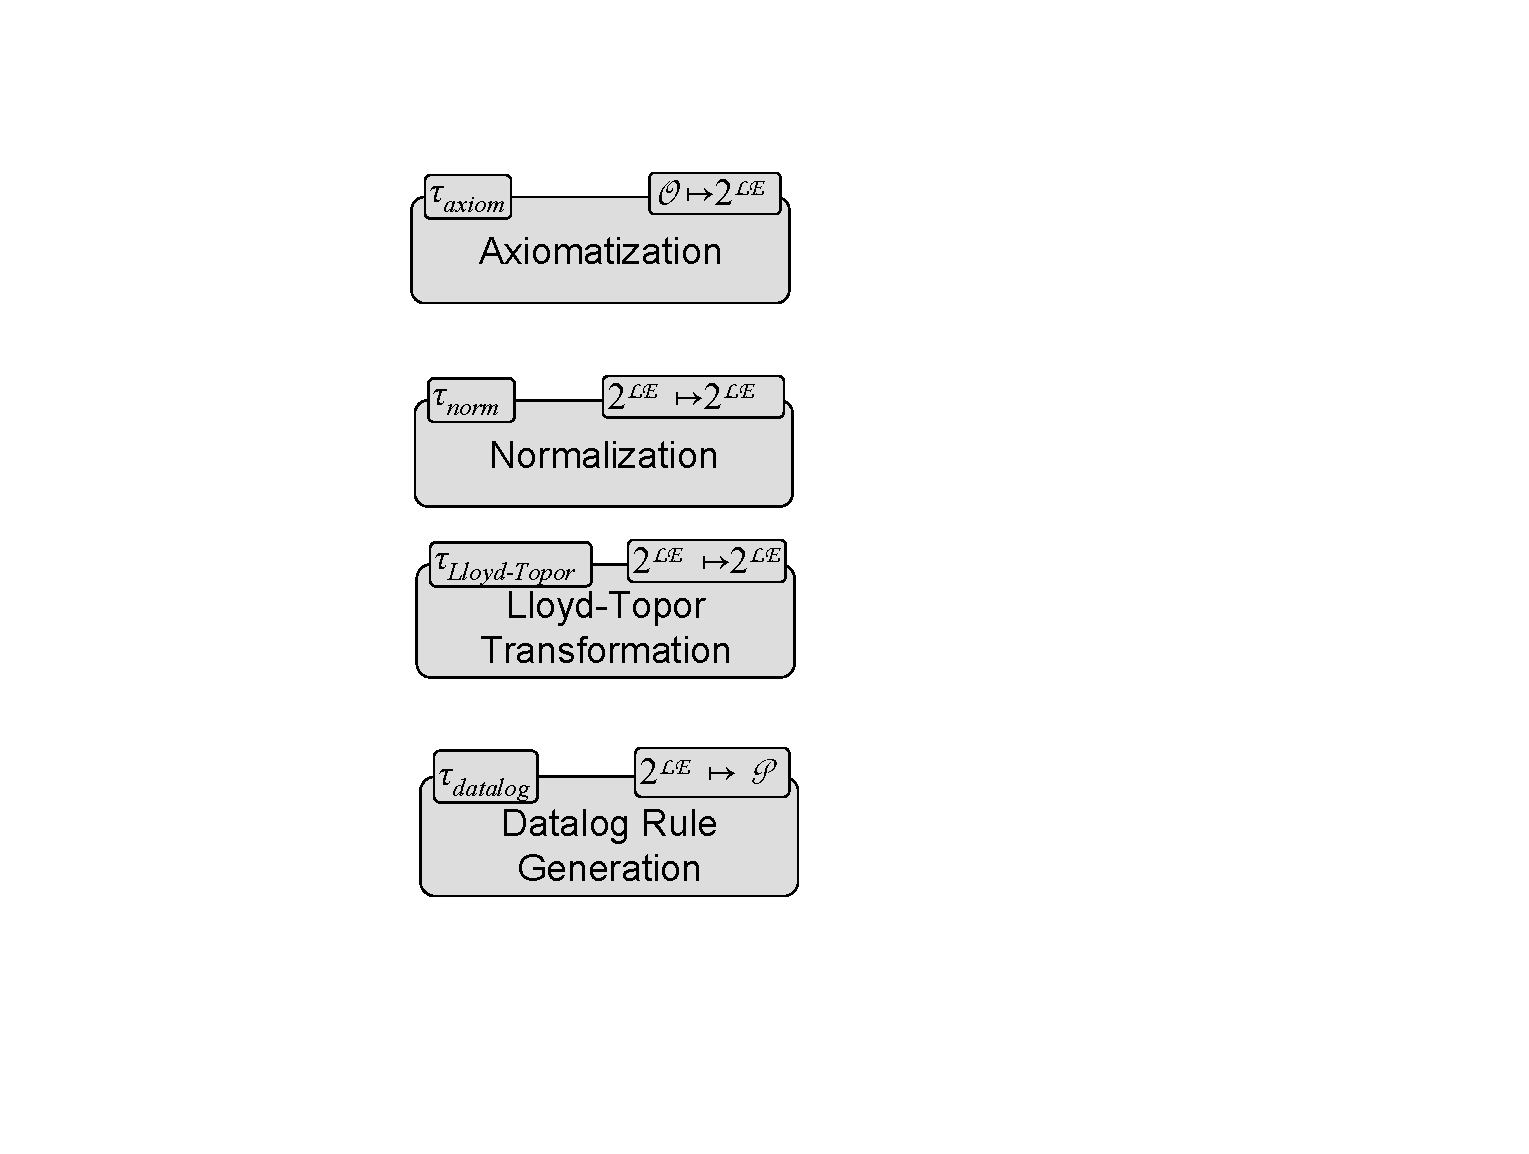
\includegraphics[width=11cm]{figures/layering}
    \centering
    \caption{Layering of the Internal Architecture. \label{fig:layering}}
\end{figure}


\subsection{Interface and Integration with Existing Technology}
So far we have not detailed on what data structure the framework
operates on. One could implement it directly with a parser and
compiler framework that generates some abstract syntax tree for WSML
which is directly transformed to the target format (Datalog).
Although this would have performance advantages, it would greatly
reduce reusability and would make maintenance harder. Our framework is
based on an intermediate object model of the language that is
provided by the WSMO4J\footnote{http://wsmo4j.sourceforge.net}
project. WSMO4J performs the task of parsing and validating WSML ontologies and provides the source object model for our translations. In order to enable the usage of different Datalog
engines we additionally implemented a simple object model for
Datalog that is independent from any particular
engine.

The main Datalog engine we used during our work was the KAON2
inference engine\footnote{KAON2 is available for download from
\url{http://kaon2.semanticweb.org}} \cite{hustadt04reducing}. As we have seen in Section~\ref{sec:datatype_reasoning}, datatype reasoning poses the biggest challenge for the Datalog implementation.
KAON2 provides a very flexible type system that allows for
user-defined datatypes, together with user-defined predicates on
these datatypes, including type checking predicates. Therefore,
KAON2 meets the identified requirements easily. As a matter of
fact, KAON2 already provided most of the required datatypes and
predicates out of the box.

{\bf GN: Perhaps we should include something about MINS?}

\section{A Use Case Example for Reasoning with WSML Ontologies\label{sec:usecase}}
-- present a WSML example ontology that demonstrates the style of modelling in rule-based WSML, to give the reader an impression what he can do with the reasoning framework \\
\phantom{mm} -- -- how do constraints work \\
\phantom{mm} -- -- how do derivation rules work \\
\phantom{mm} -- -- how does debugging support ontology development \\
-- a candidate example is the WP8 telecom bundle scenario from the last DIP review \\

\section{Outlook\label{sec:outlook}}
-- mention the planned use of KAON2's DL-capabilities for future extensions in the direction of WSML-DL \\
-- \dots


\bibliographystyle{plain}
\bibliography{paper}

\end{document}
